% !TeX root = ../../../main.tex
\subsection{Introduction}
\label{ch06:sec:intro}

The Third International Consensus Definitions for Sepsis (Sepsis-3) are the benchmark definitions for sepsis, the dysfunctional immune response to an infection, which are used in trial eligibility criteria \citep{kyriazopoulou2021procalcitonin} and phenotyping studies \citep{ch06:seymour2019derivation}.
In the critical care literature, sepsis is seen as a heterogeneous disease, a pathway arrived upon from a multitude of infectious origins, anatomical sites, and comorbid profiles.  
There is increasing recognition of the importance of time in understanding sepsis and sepsis progression, as seen in early-warning systems \citep{henry2022factors}, variation in prediction utility \citep{kamran2024evaluation}, and endotype characterization \citep{ch06:noroozizadeh2023temporal}.

Meanwhile, structured data streams, which are the data resources these tools use, are often incomplete records with insufficient information to render or confirm a diagnosis of sepsis \citep{moldwin2021empirical}. %
A more complete alternative is the discharge summary, or more generally, the case report, in which a clinician documents the clinical findings pertinent to the case and care management.
The impracticality of using the case report is that it is only written in full after the encounter is over, \emph{i.e.}, with a less granular timestamp than the events contained within. 
In principle, having a more complete, fine-grained temporal record could enable better temporal analyses of patients with sepsis, leading to better understanding and treatment improvements.

At present, the (semi-)public critical care repositories at the research frontier contain high resolution structured signals and low resolution textual signals. 
While several concerted efforts have focused on extracting temporal information, they have largely focused on temporal relations between clinical concepts \citep{sun2013evaluating} rather than on event timing.  
Those that have focused on timing \citep{leeuwenberg2020towards,ch06:frattallone2024using} used excerpted summaries and relatively small sample sizes. 


In order to train sepsis models that can incorporate information referenced in free text with finer temporal granularity, we seek to generate larger samples of textual time series.
To do so, we introduce a novel Sepsis-3 textual time series corpus from the PubMed Open Access (PMOA) Subset.
We adopt an LLM-as-annotator approach, evaluating both the ability of models to extract clinical findings and their ability to associate those findings with timestamps.
We augment existing clinical annotations with our own PMOA annotations and contrast LLM annotations with both our clinician annotations and the annotations of \cite{ch06:frattallone2024using}.
Because the corpus is automatically generated beyond the manually annotated subset, we validate it through a multi-layer framework: clinician-annotated gold-standard evaluation on \texttt{sepsis-40}, clinician--clinician agreement, bootstrap uncertainty quantification, bronze-standard proxy-reference evaluation on \texttt{sepsis-100}, direct hallucination auditing, multi-pass self-consistency, and full-corpus cross-model agreement.
These assessments provide evidence for the quality and limitations of the LLM annotations and support the use of T2S2 as a retrospective research resource for temporal modeling of sepsis trajectories.


% !TeX root = ../../../main.tex
\begin{figure}[htbp]
\begin{ChSixFloatBody}

\begin{minipage}[t]{\dimexpr \textwidth\relax}\centering

  \begin{minipage}[t]{0.65\textwidth}\vspace{0pt}
    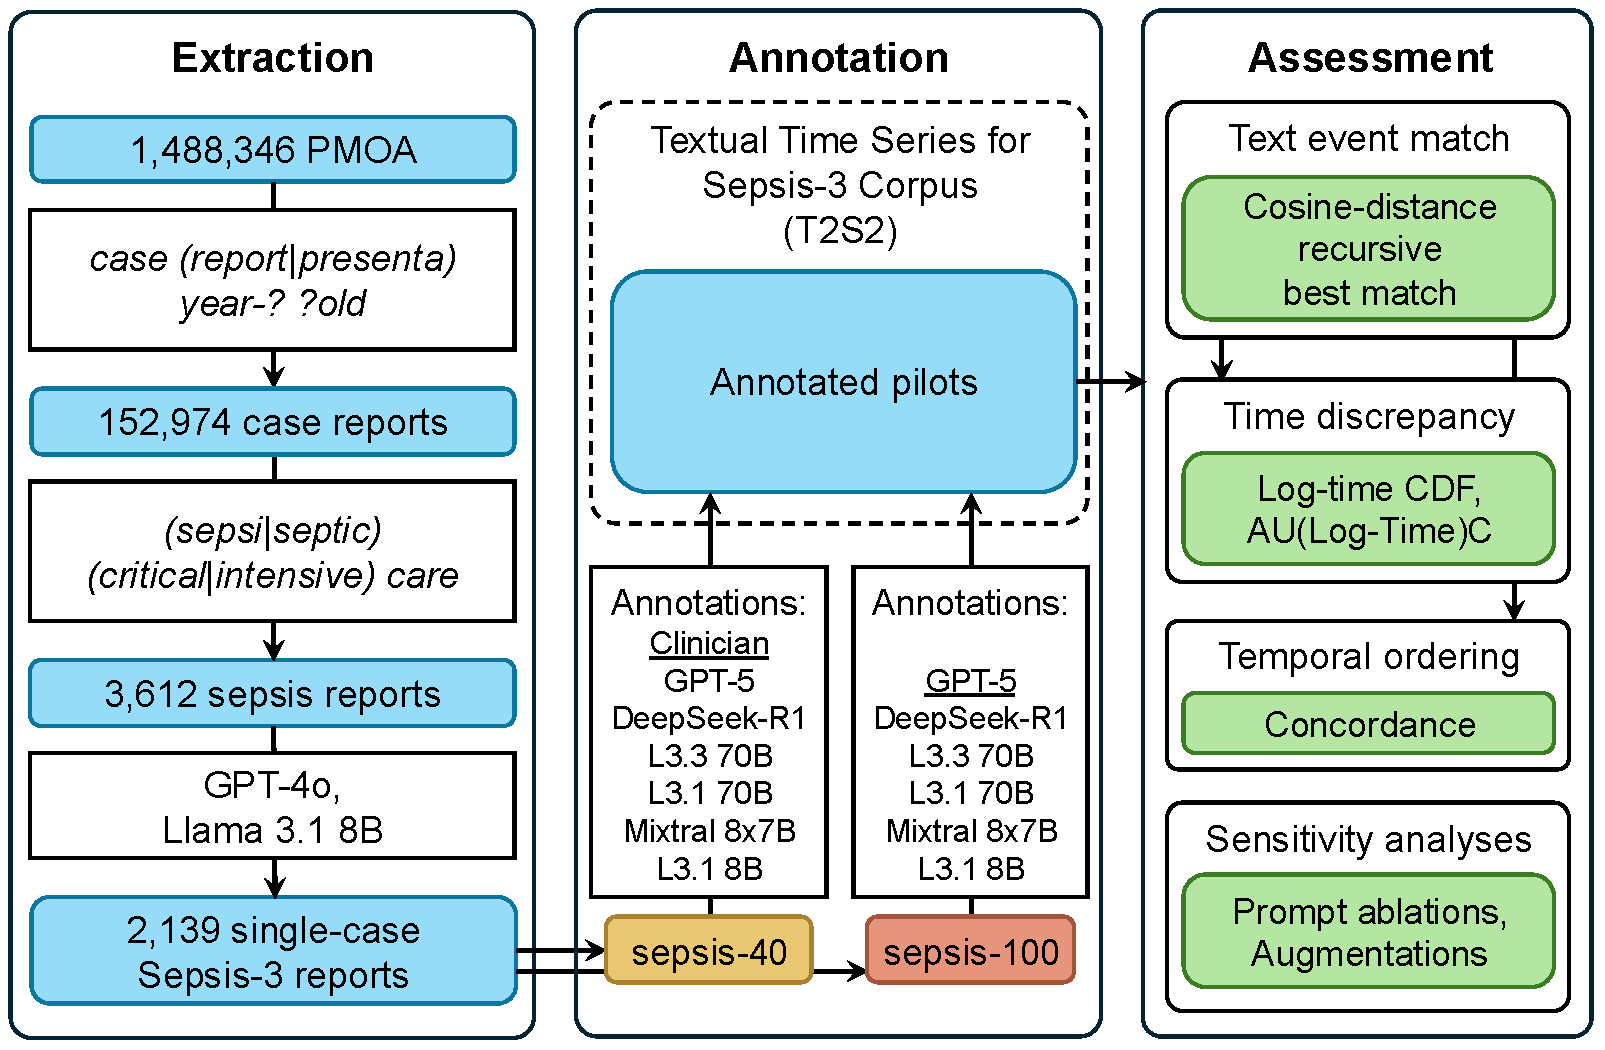
\includegraphics[width=\linewidth]{Chapters/chapter-06/images/figures/T2S2-CHIL-Main-Figure.pdf}
  \end{minipage}%
  \hspace{.5em}
  \begin{minipage}[t]{0.30\textwidth}\vspace{0pt}
    \begin{adjustbox}{max width=\linewidth}\begin{tabular}{r|cc}
    \multicolumn{3}{c}{\textbf{i2m4}} \\
    \midrule
    Qwen\textbackslash Human & Yes & No \\
    Yes & 2 & 0 \\
    No  & 0 & 18 \\
    \toprule
    L3.1 8B & Yes & No \\
    Yes & 2 & 7 \\
    No  & 0 & 11 \\
    \midrule
    \multicolumn{3}{c}{\textbf{\texttt{sepsis-100}}} \\
    \toprule
    GPT-4o\textbackslash Qwen & Yes & No \\
    Yes & 78 & 7 \\
    No  & 8 & 7 \\
    \toprule
    L3.1 8B & Yes & No \\
    Yes & 81 & 12 \\
    No  & 5 & 2 \\
    \bottomrule
    \end{tabular}\end{adjustbox}
  \end{minipage}

  
  
  
  
\end{minipage}

\end{ChSixFloatBody}
\caption{Flowchart of the PMOA T2S2 corpus construction pipeline (left).
    Confusion matrices (right) for Sepsis-3 phenotype in i2m4 (top) and \texttt{sepsis-100} (bottom) datasets, with preferred annotator in column position.}\ChSixFloatLabel{ch06:fig:flow}
\end{figure}


